\newpage
\part{Bandits-manchots}

\section{Description du probl\`eme}
On consid\`ere le probl\`eme d'apprentissage par renforcement suivant. Un agent est confront\'e \`a plusieurs reprises \`a un choix parmi $N$ diff\'erentes actions dont la r\'ecompense moyenne, notée $\mu^{i}$ pour l'action $i$, est inconnue de l'agent. 
Nous d\'esignons l'action sélectionnée sur le pas de temps $t$ par $a_{t}$, la r\'ecompense correspondante par $r_{t}$ et le nombre de fois où l’action $a$ a \'et\'e choisie jusqu'au temps $T$ par $N_{T}(a)$. 

L'objectif de l'agent est de maximiser la somme des r\'ecompenses obtenues après la période d'apprentissage, i.e.\ les $T$ premières parties. 
Autrement dit, l'agent doit identifier l'action au rendement le plus elev\'e $i^{*}$= $\argmax_{i \in {1,\dotsc,N}}\mu^{i}$ qu'il jouera continument par la suite. 
Cependant, les valeurs $\mu^{i}$ étant inconnues, il est donc contraint d'estimer ces récompenses moyennes, notée $\hat{\mu}^{i}$ pour l'action $i$, au moyen desdites parties d'apprentissage. Ces estimations sont ainsi données par :
\begin{equation*}
\hat{\mu}^{i} = \frac{1}{N_{T}(a)}\sum_{t=1}^{T} r_{t}\mathbbm{1}_{a_{t} = a}
\end{equation*}

\section{Algorithmes}
Si de nombreux algorithmes ont \'et\'e propos\'es pour r\'esoudre ce dilemme, on se contentera ici d'en citer que quelques-uns:
\subsection{Algorithme al\'eatoire}
L'algorithme al\'eatoire se contente de choisir une action uniform\'ement au hasard et il effectue ainsi uniquement de l'exploration. De ce fait, nous l'utilisons comme baseline pour les tests présentés par la suite. On peut donc d\'ej\`a pr\'esager que cet algorithme sera forc\'ement le moins optimal.

\subsection{Algorithme \textit{greedy}}
L'algorithme \textit{greedy} est bas\'e sur une politique de selection tr\`es simple qui consiste \`a s\'electionner l'une des actions ayant la valeur estim\'ee la plus \'elev\'ee :
$a_{t}$ = $\argmax_{i \in {1,\dotsc,N}}\hat{\mu}^{i}_{t}$.
Autrement dit, l'algorithme \textit{greedy} ne fait qu'\'exploiter les connaissances dont il dispose afin de maximiser la recompense \`a un instant $t$.

\subsection{Algorithme $\varepsilon$-\textit{greedy}}
Une approche courante pour trouver un compromis exploitation/exploration est l'algorithme $\varepsilon$-\textit{greedy} qui consiste à choisir à l’instant $t$, avec une probabilit\'e $1 - \varepsilon$, l’action qui maximise le rendement moyen sur les estimations faites jusque-là et avec une probabilit\'e $\varepsilon$, une action tirée d'une distribution uniforme.
L'avantage de cet algorithme repose sur le fait que, au fur et mesure que le nombre d'étapes d'apprentissage augmente, chaque action sera choisie un très grand nombre de fois assurant ainsi que tous les $\hat{\mu}^{i}$ convergeront vers les $\mu^{i}$. 

Par ailleurs, la valeur de $\varepsilon$ a un fort impact sur l'apprentissage. C'est pour cela qu'on en a test\'e diff\'erentes valeurs (constantes) et même sous la forme d'une fonction décroissante du temps. On peut conj\'ecturer la puissance de cet algorithme et sa capacit\'e à explorer toutes les actions possibles et de prendre des d\'ecisions quasi proches de l’optimum.

\subsection{Algorithme \textit{Upper Confidence Bound}}
L'algorithme UCB est une autre strat\'egie qui permet de trouver une balance entre l'exploration et l'exploitation. L'id\'ee de l'algorithme consiste \`a se fier des estimations faites jusqu'alors \`a une borne sup\'erieure de confiance. En effet, une incertitude existera toujours sur l'optimalit\'e de ces estimations. 

Les deux algorithmes d\'efinis pr\'ecédemment choisissent toujours l'action qui semble meilleure \`a un instant $t$ ou se contentent de choisir des actions al\'eatoirement sans distinction. L'algorithme UCB prend en revanche en compte l'optimalit\'e des estimations mais également l'incertitude sur celles-ci. Il sélectionne l'action : $a_{t}$ = $\argmax_{i \in {1,\ldots,N}}(\hat{\mu}^{i}_{t} + \sqrt{\frac{2\log(t)}{N_{T}(i)}})$.
L'incertitude est mesur\'ee par le deuxi\`eme terme, il permet notamment de privil\'egier les actions le plus d\'efavoris\'ees par les choix de l'agent.
\newpage
\section{Mise en oeuvre et expérimentations}

\begin{figure}[!h]
\centering
  \begin{center}
    \subfloat[Regret cumulé][Regret cumulé en fonction du nombre d'étapes d'apprentissage]{
      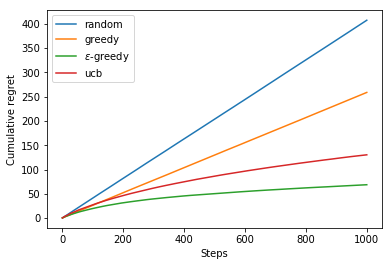
\includegraphics[width=0.5\textwidth]{Project_1/Report/sections/Figures/cum_regret.png}
      \label{sub:}
                         }
    \subfloat[Récompense cumulée][Récompense cumulée en fonction du nombre d'étapes d'apprentissage]{
      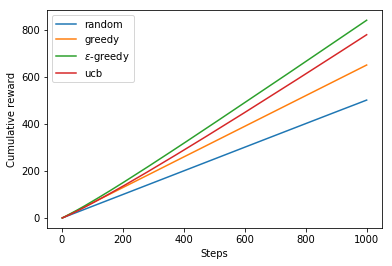
\includegraphics[width=0.5\textwidth]{Project_1/Report/sections/Figures/cum_reward.png}
      \label{sub:}
                        }
    \caption[Performance des algorithmes pour la machine à leviers]{Performance des quatres algorithmes sur 10 leviers et 2000 exécutions}
    \label{fig:}
  \end{center}
\end{figure}

La figure 1 montre le gain et le regret cumulé en fonction de $t$ pour les quatre algorithmes décrits dans la section précédente. Nous avons fait le choix de simuler avec une machine à 10 léviers, chacun d'entre eux suivant une loi de Bernoulli avec un paramètre choisi uniformément dans [0,1].

Comme dit précédemment, les algorithmes aléatoire et \textit{greedy} correspondent respectivement aux comportements purement exploratoire et d'exploitation. Les courbes confirment ainsi nos hypothèses de départ, à savoir que ces comportements amèneraient à des résultats sous-optimaux, voire mauvais. 

En revanche, les deux autres algorithmes trouvent un équilibre entre les deux comportements au taux d'équilibre entre l'exploration et l'exploitation près ; c'est pourquoi les résultats sont plus intéressants.
Cependant, le taux d'équilibre utilisé n'est pas le même dans les deux cas. En effet, l'algorithme $\varepsilon$-\textit{greedy} ($\varepsilon = 0.04$) choisit des actions au hasard dans 4 \% des cas, ce qui reste un taux assez bas. Ceci contraste avec la "méfiance" de l'algorithme UCB en ses connaissances, ce qui le fait garder un comportement plus exploratoire dans le temps. Nous pouvons voir ces différences dans les valeurs $N_T(a)$ : pour UCB, l'écart entre elles reste réduit en raison de sa "méfiance", alors que pour $\varepsilon$-\textit{greedy}, d'après son trait d'exploitation, il y a une (ou très peu de) valeur qui est beaucoup plus élevée que les autres.

\begin{figure}[ht]
\centering
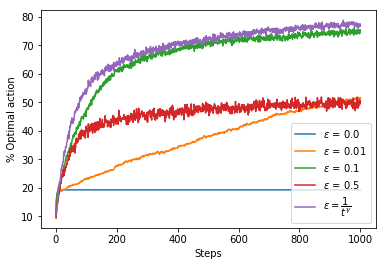
\includegraphics[width=0.6\textwidth]{Project_1/Report/sections/Figures/eps_variable_ok.png}
\caption{Pourcentage de choix du meilleur levier par $\varepsilon$-\textit{greedy}}
\label{FigGraphes}
\end{figure}

Par ailleurs, le comportement exploratoire constant dans le temps de l'algorithme $\varepsilon$-\textit{greedy} reste un choix raisonnable au vu de la figure 2. Nous pouvons y apprécier que, malgré ses choix sous-optimaux dans les $200$ premiers pas, il arrive à de résultats aussi bons, notamment pour $\varepsilon = 0.1$, que ceux de la méthode avec $\varepsilon = \frac{1}{t^{0.35}}$, i.e.\ décroissant dans le temps.

\begin{figure}[!h]
\centering
  \begin{center}
    \subfloat[Sans écart fixé]{
      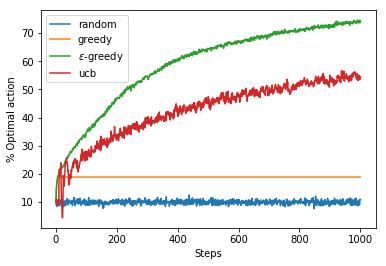
\includegraphics[width=0.5\textwidth]{Project_1/Report/sections/Figures/proportion_0_0.png}
      \label{sub:}
                         }
    \subfloat[\'Ecart de 25 \%]{
      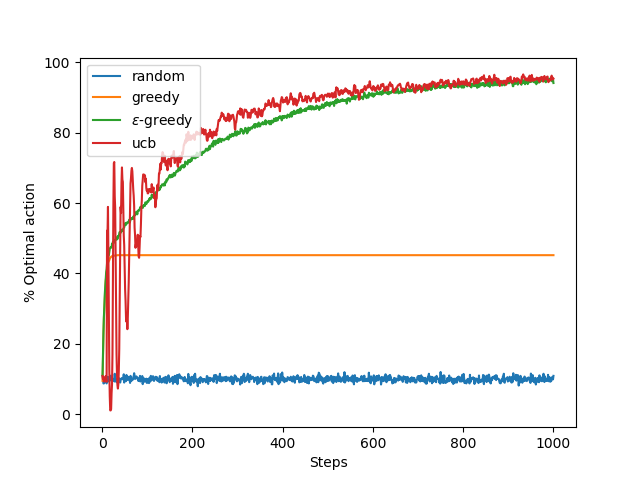
\includegraphics[width=0.5\textwidth]{Project_1/Report/sections/Figures/proportion_0_25.png}
      \label{sub:}
                        }
    \newline
    \subfloat[\'Ecart de 50 \%]{
      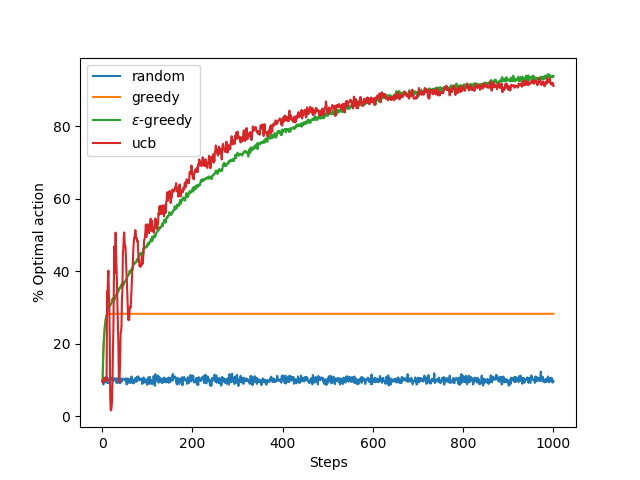
\includegraphics[width=0.5\textwidth]{Project_1/Report/sections/Figures/proportion_0_50.png}
      \label{sub:}
                         }
    \subfloat[\'Ecart de 75 \%]{
      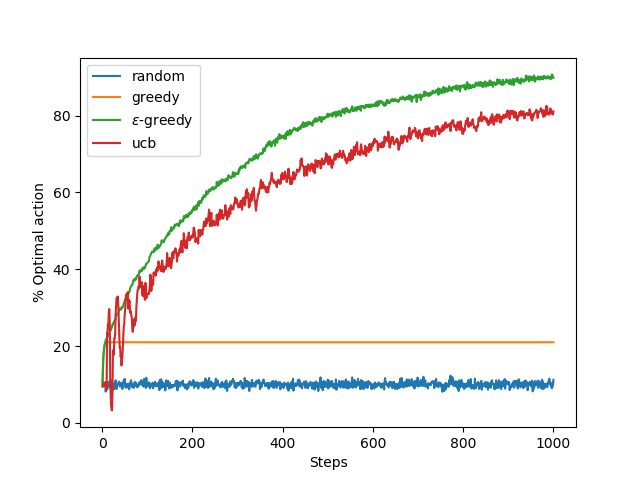
\includegraphics[width=0.5\textwidth]{Project_1/Report/sections/Figures/proportion_0_75.png}
      \label{sub:}
                        }
    \caption[Mesure de performance selon l'écart dans la distribution de récompenses moyennes]{Performance des quatres algorithmes sur $1000$ pas d'apprentissage et $2000$ exécutions pour différentes proportions entre les deux meilleures récompenses moyennes}
    \label{fig:}
  \end{center}
\end{figure}

La figure 3 montre l'impact de l'écart entre la meilleure récompense de la machine et la deuxième meilleure sur la performance des algorithmes.
Pour l'algorithme aléatoire, cela reste identique dans les quatre cas car il ne possède aucune dépendance.
Pour l'algorithme \textit{greedy}, nous savons qu'il choisit une première action de manière aléatoire (car les estimations sont toutes initialisées à $0$), et la garde tout au long de l'apprentissage. C'est pourquoi, pour un écart donné, le nombre de choix optimaux reste constant, mais, lorsque nous considérons l'ensemble d'écarts, les valeurs obtenues ne sont pas dépendantes les unes des autres.

Pour les deux autres algorithmes, comme ils possèdent un trait exploratoire, l'écart dans la distribution des récompenses a un effet remarquable. D'un côté, l'algorithme $\varepsilon$-\textit{greedy} améliore ses performances car, dès la reconnaissance du meilleur levier, il le choisit majoritairement. D'autre côté, pour l'algorithme UCB, il y a un pourcentage d'écart optimal qui se trouve entre 25 \% et 50 \% : tout comme pour l'algorithme $\varepsilon$-\textit{greedy}, son trait d'exploitation fait qu'il améliore ses performances, mais, comme déjà mentionné, il effectue plus d'exploration que ce dernier et il continue à ce faire même lorsqu'il a trouvé le meilleur levier. Dans ce cas-là, nous disons que l'algorithme cherche à améliorer ses connaissances déjà optimales.

\begin{figure}[!h]
\centering
  \begin{center}
    \subfloat[Regret cumulé][Regret cumulé en fonction du nombre d'étapes d'apprentissage]{
      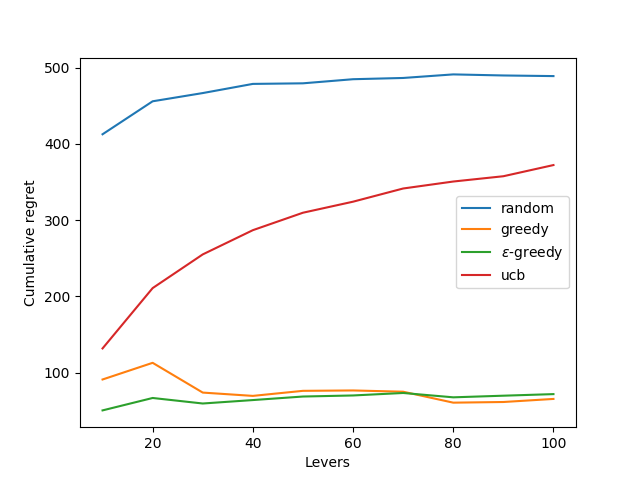
\includegraphics[width=0.5\textwidth]{Project_1/Report/sections/Figures/var_levers_cum_regret.png}
      \label{sub:}
                         }
    \subfloat[Récompense moyenne][Récompense cumulée en fonction du nombre d'étapes d'apprentissage]{
      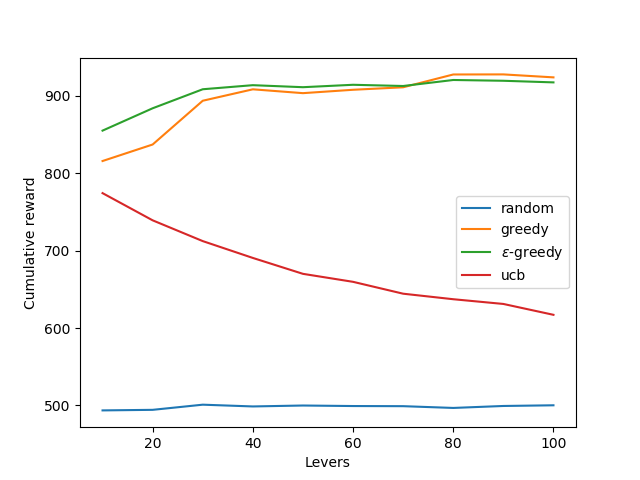
\includegraphics[width=0.5\textwidth]{Project_1/Report/sections/Figures/var_levers_cum_rew.png}
      \label{sub:}
                        }
    \newline
    \subfloat[Nombre de choix optimaux][Nombre de choix optimaux en fonction du nombre d'étapes d'apprentissage]{
      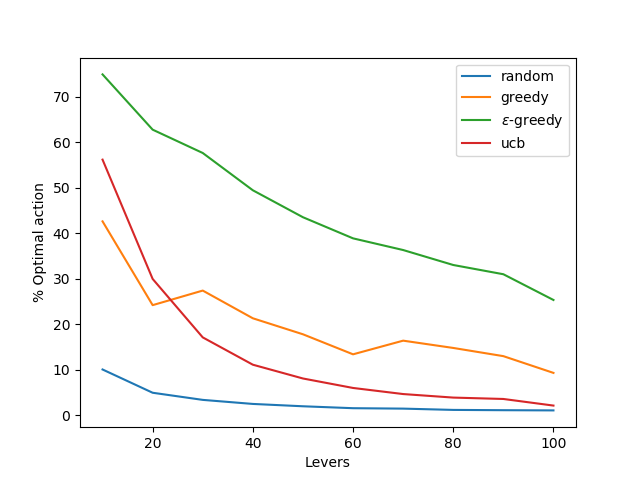
\includegraphics[width=0.5\textwidth]{Project_1/Report/sections/Figures/var_levers_opt_action.png}
      \label{sub:}
                         }
    \caption[Mesure de performance selon le nombre de leviers]{Performance des quatres algorithmes sur $1000$ pas d'apprentissage et $500$ exécutions pour différents nombres de leviers}
    \label{fig:}
  \end{center}
\end{figure}

Pour la dernière expérience sur la machine à $N$-leviers, nous avons fait varier le nombre de leviers. Pour ce faire, nous avons fixé la longueur de la période d'apprentissage à $1000$ pas et effectué $500$ exécutions avec des distributions de récompenses aléatoires. Au fur et à mesure que le nombre de leviers augmente, les agents ont moins de chances de retrouver le levier optimal avec un nombre de pas d'apprentissage fixé. Ceci explique ainsi les courbes sur la figure 4-$c$. En effet, caractère exploratoire ou pas, il y a plus de leviers à tester et ça veut dire plus de pas nécessaires.